\documentclass{beamer}
\usetheme[
  block=fill,
  background=dark,
  titleformat=smallcaps,
  progressbar=frametitle,
  numbering=none,
]{metropolis}

%----------------------------------------------------------------------------
% LoCo
%----------------------------------------------------------------------------
\setbeamertemplate{frametitle}[default][center]

%Color
\definecolor{mDarkBrown}{HTML}{604c38}
\definecolor{mDarkTeal}{HTML}{23373b}
\definecolor{mLightBrown}{HTML}{EB811B}
\definecolor{mLightGreen}{HTML}{14B03D}
% Math
\usepackage{amsmath}
\usepackage{amssymb}
\usepackage{stmaryrd}
% Code listing
\usepackage{minted}
%\usemintedstyle{friendly}
\usemintedstyle{tango}
\usepackage{algorithm}
\usepackage[noend]{algpseudocode}

% Graphs
\usepackage{tikz}
\usetikzlibrary{calc, trees, fit}
\usepackage{pgfplots}
% Graphics
\usepackage{graphics}
\graphicspath{{figures/}} % Location of the graphics files

\newcommand\todo[1]{\textcolor{red}{#1}}
\newcommand{\w}[1]{\textit{"#1"}}
\newcommand{\sm}[1]{\text{\small{#1}}}
\newcommand\s{\textsc}

% Box macro
\newcommand{\ex}[2]{
  \vfill
  \begin{alertblock}{#1}
    #2
  \end{alertblock}
}
\newcommand\tsc[1]{\alert{\textsc{#1}}}

%----------------------------------------------------------------------------

% Beamer
\title{Differentiable Neural Computers}
\subtitle{Hybrid Computing using a neural network with dynamic external memory (Graves et al. 2016)}
\author{Konstantinos Kogkalidis}
\date{May 28, 2018}
\institute{Universiteit Utrecht}

\begin{document}
	\maketitle
	
\begin{frame}{Overview}
	A \alert{recurrent neural network} controlling a large external memory.
	
	\pause
	Key Features:
	\begin{itemize}
	\item End-to-end differentiable
	\item Turing complete
	\item Extension of NTMs
	\end{itemize}
\end{frame}

\begin{frame}{Introduction: Motivation}
	\alert{Von Neumann architecture}
	\begin{figure}
	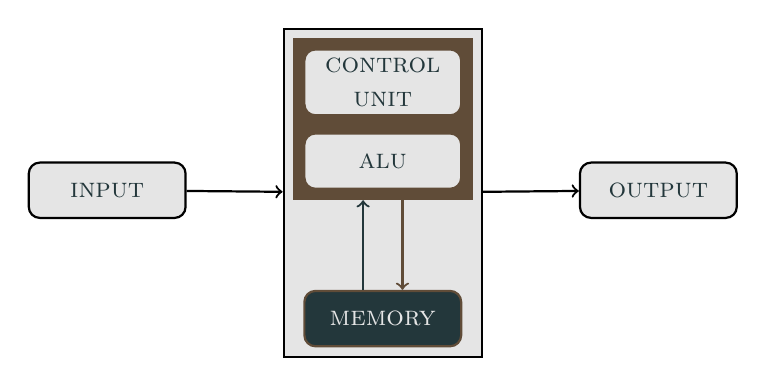
\begin{tikzpicture}
		[auto,
		block/.style ={rectangle, draw=mDarkBrown, thick, fill=gray!20, text width=5em, align=center, rounded corners, minimum height=2em},
		block2/.style ={rectangle, draw=mDarkBrown, thick, fill=mDarkTeal, text width=5em, align=center, rounded corners, minimum height=2em},
		block3/.style ={rectangle, draw=black, thick, fill=gray!20, text width=5em, align=center, rounded corners, minimum height=2em}]
		\draw (-1,0.63) node[block3] (i) {\textcolor{mDarkTeal}{\sc{input}}};
		\draw (6,0.63) node[block3] (o) {\textcolor{mDarkTeal}{\sc{output}}};
		
		\draw (2.5,-1) node[block2] (m) {\textcolor{gray!20}{\sc{memory}}};
		\draw (2.5,1) node[block] (a) {\textcolor{mDarkTeal}{\sc{alu}}};
		\draw (2.5,2) node[block] (c) {\textcolor{mDarkTeal}{\sc{control unit}}};
		
		\node[draw=mDarkBrown, thick, fill=mDarkBrown, fit=(a) (c)](Fit1) {};
		\draw (2.5,1) node[block] (a) {\textcolor{mDarkTeal}{\sc{alu}}};
		\draw (2.5,2) node[block] (c) {\textcolor{mDarkTeal}{\sc{control unit}}};
		
		\node[draw=black, thick, fill=gray!20, fit=(Fit1) (m)](Fit2) {};
		\node[draw=mDarkBrown, thick, fill=mDarkBrown, fit=(a) (c)](Fit1) {};
		\draw (2.5,1) node[block] (a) {\textcolor{mDarkTeal}{\sc{alu}}};
		\draw (2.5,2) node[block] (c) {\textcolor{mDarkTeal}{\sc{control unit}}};
		\draw (2.5,-1) node[block2] (m) {\textcolor{gray!20}{\sc{memory}}};

		\draw (i) edge [->, black, thick] (Fit2);
		\draw (Fit2) edge [->, black, thick] (o);
		\draw ($(m.north) + (0.25,0)$) edge [<-, mDarkBrown, thick] ($(Fit1.south) + (0.25, 0)$ );
		\draw ($(m.north) + (-0.25,0)$) edge [->, mDarkTeal, thick] ($(Fit1.south) + (-0.25, 0)$ );

	\end{tikzpicture}
	\end{figure}
\end{frame}

\begin{frame}{Introduction: Motivation}
	\begin{minipage}{.4\textwidth}	
	\alert{Simple Neural Net}
	\begin{figure}
	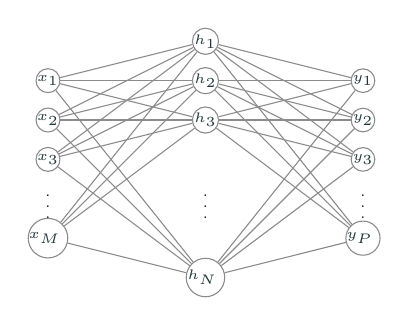
\begin{tikzpicture}[scale=.5]
		\foreach \y /\alph/\name in {
			0/x1/$x_1$,
		  	-1/x2/$x_2$,
		  	-2/x3/$x_3$,
		  	-4/xM/$x_M$
		 }{
		% 	\node[] (\alph) at (0,\y) {\name};
		 	\node[circle, draw=gray!90, inner sep=0pt,minimum size=3mm,fill=white] (\alph) at (0,\y) {\tiny \textcolor{mDarkTeal}{\name}};
		 }
		 \node (x..) at (0,-3) {\tiny {\vdots}};
		 \foreach \y /\alph/\name in {
			1/h1/$h_1$,
		  	0/h2/$h_2$,
		  	-1/h3/$h_3$,
		  	-5/hN/$h_N$
		 }{
		 	\node[circle, draw=gray!90, inner sep=0pt,minimum size=3mm,fill=white] (\alph) at (4,\y) {\tiny \textcolor{mDarkTeal}{\name}};
		 }
		 \node (h..) at (4,-3) {\tiny {\vdots}};
		 \foreach \y /\alph/\name in {
			0/y1/$y_1$,
		  	-1/y2/$y_2$,
		  	-2/y3/$y_3$,
		  	-4/yP/$y_P$
		 }{
		 	\node[circle, draw=gray!90,inner sep=0pt,minimum size=3mm,fill=white] (\alph) at (8,\y) {\tiny \textcolor{mDarkTeal}{\name}};
		 }
		 \node (y..) at (8,-3) {\tiny {\vdots}};
		 \foreach \x in {x1, x2, x3, xM}
		 {\foreach \h in {h1, h2, h3, hN}
		 {\draw (\x) edge[gray!90] (\h);}}
		 \foreach \x in {h1, h2, h3, hN}
		 {\foreach \y in {y1, y2, y3, yP}
		 {\draw (\x) edge[gray!90] (\y);}}
	\end{tikzpicture}
	\end{figure}
	\end{minipage}
	\pause
	\hspace{1cm}
	\begin{minipage}{.4\textwidth}	
	\alert{Recurrent Neural Net}
	\begin{figure}
	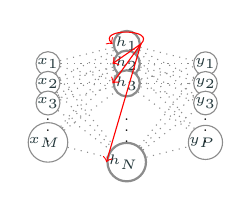
\begin{tikzpicture}[scale=.25]
		\foreach \y /\alph/\name in {
			0/x1/$x_1$,
		  	-1/x2/$x_2$,
		  	-2/x3/$x_3$,
		  	-4/xM/$x_M$
		 }{
		% 	\node[] (\alph) at (0,\y) {\name};
		 	\node[circle, draw=gray!90, inner sep=0pt,minimum size=3mm,fill=white] (\alph) at (0,\y) {\tiny \textcolor{mDarkTeal}{\name}};
		 }
		 \node (x..) at (0,-3) {\tiny {\vdots}};
		 \foreach \y /\alph/\name in {
			1/h1/$h_1$,
		  	0/h2/$h_2$,
		  	-1/h3/$h_3$,
		  	-5/hN/$h_N$
		 }{
		 	\node[circle, draw=gray!90, thick, inner sep=0pt,minimum size=3mm,fill=white] (\alph) at (4,\y) {\tiny \textcolor{mDarkTeal}{\name}};
		 }
		 \node (h..) at (4,-3) {\tiny {\vdots}};
		 \foreach \y /\alph/\name in {
			0/y1/$y_1$,
		  	-1/y2/$y_2$,
		  	-2/y3/$y_3$,
		  	-4/yP/$y_P$
		 }{
		 	\node[circle, draw=gray!90, inner sep=0pt,minimum size=3mm,fill=white] (\alph) at (8,\y) {\tiny \textcolor{mDarkTeal}{\name}};
		 }
		 \node (y..) at (8,-3) {\tiny {\vdots}};
		 \foreach \x in {x1, x2, x3, xM}
		 {\foreach \h in {h1, h2, h3, hN}
		 {\draw (\x) edge[dotted, gray!90] (\h);}}
		 \foreach \x in {h1, h2, h3, hN}
		 {\foreach \y in {y1, y2, y3, yP}
		 {\draw (\x) edge[dotted, gray!90] (\y);}}
		 \foreach \h in {h1}
		 {\draw (\h.west) [<-, red] .. controls +(-0.8,0.8) and +(0.8,0.8) .. (\h.east);}
		 \foreach \h in {h1}
		 {\foreach \hh in {h2, h3, hN}
		 {\draw (\h.east) edge[->, red] (\hh.west);}}
	\end{tikzpicture}
	\end{figure}
	\end{minipage}
\end{frame}

	
\end{document}
